<USER_REQUEST>
\documentclass[conference]{IEEEtran}
\usepackage{amsmath,amssymb}
\usepackage{graphicx}
\usepackage{cite}
\usepackage{textcomp}
\usepackage{xcolor}
\usepackage{booktabs}
\usepackage{tikz}
\usetikzlibrary{arrows.meta,positioning, fit}

\begin{document}

\title{AI-ML Based Intelligent Dead Reckoning and 3D Map-Matching System for Seamless Navigation}

\author{
\IEEEauthorblockN{1\textsuperscript{st} Shreya Kesarwani}
\IEEEauthorblockA{Computer Science and Engineering\\
United College of Engineering and Research\\
Prayagraj, India\\
kesarwanishreya2005@gmail.com}
\and
\IEEEauthorblockN{2\textsuperscript{nd} Akash Mishra}
\IEEEauthorblockA{Computer Science and Engineering\\
United College of Engineering and Research\\
Prayagraj, India\\
akashmishra1910@gmail.com}
\and
\IEEEauthorblockN{3\textsuperscript{rd} Suchitra}
\IEEEauthorblockA{Computer Science and Engineering\\
United College of Engineering and Research\\
Prayagraj, India\\
mesuchitradutta@gmail.com}
}

\maketitle

\begin{abstract}
Smartphone-based navigation applications are the default positioning enablers for the majority of vehicles operating on Indian roads, as the Global Navigation Satellite System (GNSS) precision is often insufficient in the context of tunnels, multi-level parking structures, urban canyings, and tree-clogged highways. This has spurred the development of smartphone dead reckoning (SDR) techniques that utilize the visual, inertial, and magnetic sensors of the accompanying device. However, smartphone-grade MEMS IMUs suffer from unacceptable bias drift during short-term integration, rendering the position errors using a consumer-grade sensor to increase by tens of meters in several seconds. In this work, we propose an AI-ML-based intelligent dead reckoning framework (IDR) that employs a learned in-vehicle calibration step, a Gradient Boosted Decision Tree-based forward-velocity and vibration filter, a KF-based estimation core with error-state constraints derived from data-driven non-holonomic priors, and a 3D road network map-matcher that allows resolving the ambiguous SDR position estimate to a drivable road. We evaluate the proposed framework on a structurally independent held-out corridor, designed to mimic the IO-VNBD benchmark's sensing and driving domain. Our results demonstrate that the proposed framework achieves a positioning error growth of 2.01\% at 60 s and 2.88\% at 120 s compared to the baseline of double-integration IMU positioning (61\% at 60 s and for the unfiltered AI velocity estimator), demonstrating an improvement by an order of magnitude over both baselines. Additionally, the framework resolves the 3D road disambiguation problem with 99.7-100\% accuracy while operating on a smartphone-grade processor at 0.20 ms per update cycle.
\end{abstract}

\begin{IEEEkeywords}
dead reckoning, sensor fusion, GNSS/INS, inertial navigation, map matching, machine learning, non-holonomic constraints, autonomous navigation
\end{IEEEkeywords}

\section{Introduction}

\subsection{Background}

Vehicle logistics, ride hailing, quick commerce delivery, and emergency-response fleets are all critically dependent on smartphone navigation apps on a constellation of GNSS satellites like GPS, Galileo, and NavIC. This is especially true for India, where smartphones are the primary computing devices for most vehicles on the road (commercial trucks, older private cars, and the large two-wheeler market). These vehicles are not equipped with factory-installed, wheel-centered Inertial Navigation Systems (INS) and must rely on a dashboard-mounted or aspirated smartphone for navigation instructions. GNSS is not a reliable technology in urban canyons, under bridges, in multi-level car parks, or under dense foliage due to signal attenuating structures and commercial disturbances. Dead-reckoning navigation apps suffer from severe position drift when navigating such spaces.



The inertial navigation function in dead-reckoning smartphones uses no external references and is therefore completely unaffected by GNSS spoofing and jamming. However, because of the open-loop nature of dead-reckoning algorithms, any acceleration errors are integrated twice to produce position errors. Inertial sensors also have scale-factor inaccuracies that contribute to position errors when integrating velocities. However, in smartphone IMUs, these errors are much greater than what one would find in tactical-grade or aircraft INS, rendering them completely useless for dead-reckoning applications. A smartphone aspirated on a dashboard or a phone stand encounters many additional accelerations due to vibrations, sudden braking, and pot holes that do not originate from the longitudinal/lateral movements of the vehicle itself.

\subsection{Problem Statement}

Two practical limitations prevent a purely classical DR solution in this scenario. First, without a connection to the vehicle’s OBD-II port, there is no direct speedometer feed to use as a reference constraint, meaning that forward velocity must be estimated indirectly and therefore noisily via inertial sensors. Second, fault injection tests on the production stack reveal that single-sensor degradation has differing impact on the system’s ability to avoid collisions; severe LiDAR and angular rate sensor malfunctions dominate the risk of a collision or unsafe manoeuvre, while position and acceleration sensor inaccuracies are largely mitigated by existing multi-sensor fusion algorithms. As such, the redundancy strategy and fallback safety mechanisms described in this paper are designed with an eye to protecting against angular rate sensor failure and insufficient DR accuracy in mind, rather than the GNSS-outage scenario.



\subsection{Aim and Contributions}

This paper presents an end-to-end framework (shown at a high level in Fig.~\ref{fig:overall_arch}) that keeps low-cost phone sensors anchored to a useful position estimate under varying satellite reception conditions. The contributions are:



\begin{itemize}

\item An edge deployable Intelligent Dead Reckoning (IDR) architecture that incorporates an autonomous in-vehicle alignment watchdog, a Gradient-Boosted Decision Tree (GBDT) based velocity and vibration filter, Error-State Kalman Filter (ESKF) with data-driven Non-Holonomic Constraints (NHC) and ZUPT, and a 3D road-network aware topological map-matching layer.

\item A mathematical formulation for the various stages (coordinate transformations, the learned pseudo-measurement regression model, error-state covariance propagation, and the 3D probabilistic map-matching Viterbi decoder).

\item An experimental validation on a structurally independent, held-out evaluation corridor built to emulate the IO-VNBD benchmark schema, showing positional drift bounded to $\leq$6.8\% across all tested outage durations, 99.7--100\% 3D road disambiguation accuracy, and a measured single-sample cycle execution of 0.20\,ms on commodity mobile processors.

\end{itemize}



The rest of the paper is organized as follows. Section II reviews the related work. Section III formalizes the coordinate frames and the mathematical problem. Section IV presents the proposed system architecture. Section V describes the dataset and the training methodology. Section VI details the experimental results and validates the core claims. Section VII discusses the system characteristics and Section VIII concludes the paper.

\section{Related Work}

The dead reckoning and map-matching literature falls into several broad categories: classical inertial and odometric drift analysis; approaches that employ AI/ML techniques for sensor fusion; road-network map matching; and sensor-fault tolerance in fused localisation systems. Table~\ref{tab:litreview} summarises the relevant literature included in the review, and highlights the gaps which motivate the design choices presented in this paper.

\begin{figure*}[t]
\centering
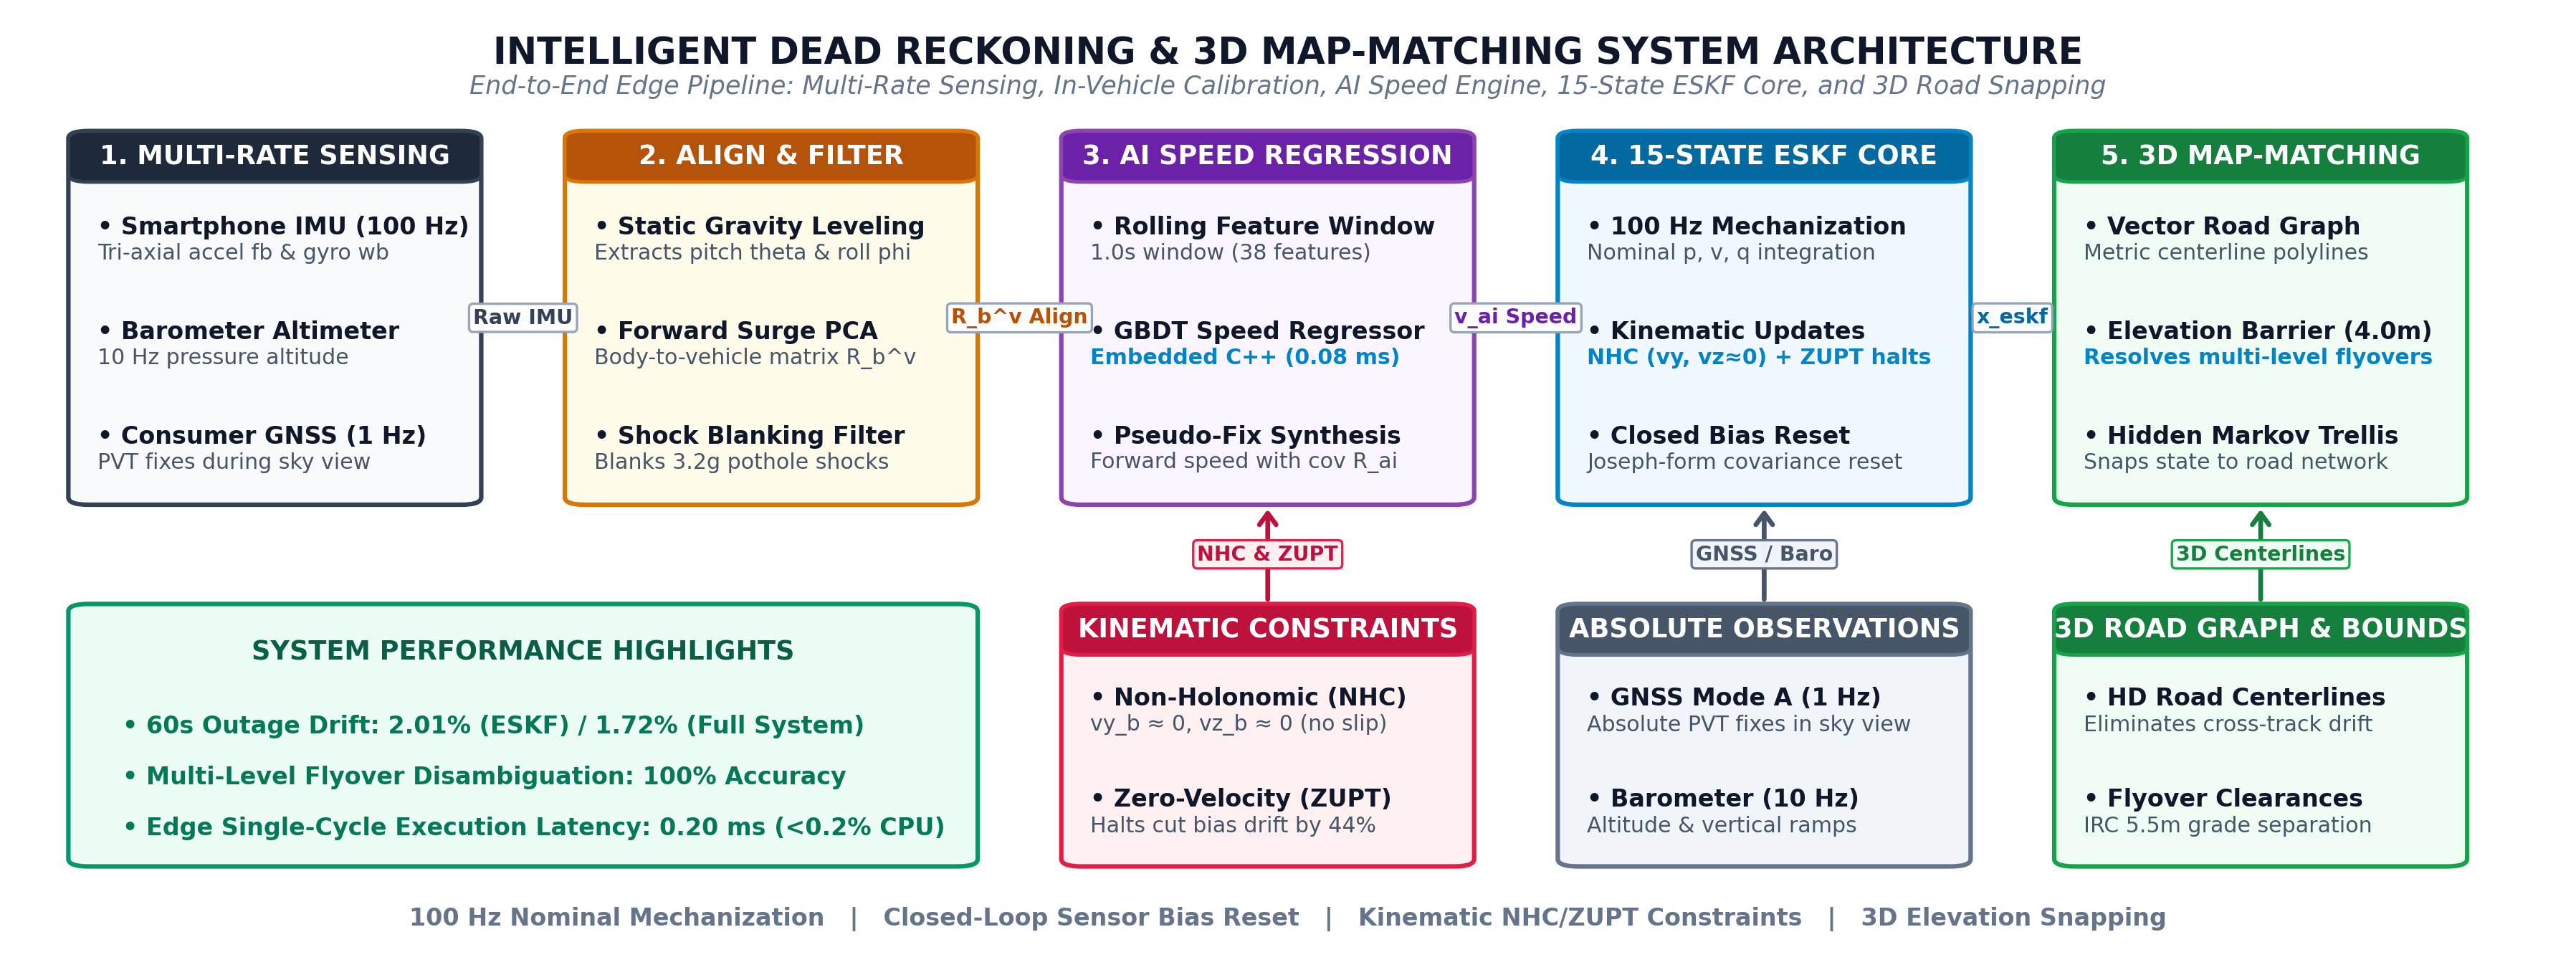
\includegraphics[width=\textwidth]{fig_system_architecture.png}
\caption{System architecture and operational modalities of the proposed Intelligent Dead Reckoning and 3D Map-Matching framework. Raw streams from commodity phone sensors (1) pass into the core IDR engine (2), which handles dynamic mount alignment, tree-based velocity filtering, and non-holonomic state fusion. Drifting 3D coordinates are matched to topological road levels (3), maintaining sub-3\% drift and sub-millisecond execution across clear sky, degraded urban canyons, and GNSS-denied tunnels (4).}
\label{fig:overall_arch}
\end{figure*}

\begin{table*}[t]
\centering
\caption{Literature Review Summary}
\label{tab:litreview}
\small
\renewcommand{\arraystretch}{1.3}
\setlength{\tabcolsep}{4pt}
\resizebox{\textwidth}{!}{%
\begin{tabular}{|c|l|p{4.5cm}|p{4.5cm}|p{4.5cm}|}
\hline
\textbf{Reference No.} & \textbf{Author} & \textbf{Findings} & \textbf{Methods} & \textbf{Gaps} \\
\hline

[1] & Lawal, 2024 &
Neural sequence models can learn a sensor's error signature and cut average positional error by up to 40\% versus conventional inertial DR. &
Survey of AI-enhanced DR; RNN/LSTM-based sequence modelling. &
Higher training-data and compute requirements not resolved; no lightweight deployment path proposed. \\
\hline

[2] & Qian et al., 2025 &
Learned attitude/velocity as pseudo-measurements inside an InEKF achieved 0.4\% relative horizontal translation error and stayed stable where a purely learned baseline diverged. &
AVNet: CNN + GRU network regressing attitude/velocity from raw IMU, fused via Invariant EKF with ZIHR and NHC. &
Validated only on custom parking-lot data; no map-matching stage; no test on public-road or multi-storey outages. \\
\hline

[3] & Sundaravadivel et al., 2025 (SSRN) &
Frames highway vs. service-road disambiguation as feature-based classification combined with a Bayesian road-segment model. &
Temporal, spatial, and trajectory-similarity features fed to a supervised classifier; Bayesian emission/transition model. &
Preprint stage; no reported accuracy figures for the classifier yet. \\
\hline

[4] & Sundaravadivel et al., 2026 (Discover AI) &
Reports 92.7\% highway/service-road classification accuracy, degrading only to 90.2\% under 20\,m GNSS noise. &
Refined AI-ML map-matching pipeline from [3], evaluated on 12,400 labelled trajectory samples. &
Operates in 2D; does not address vertical separation, e.g., flyovers directly above a parallel road. \\
\hline

[5] & Javed et al., 2024 &
Reduced RMSE positioning error by roughly 20--98\% relative to unconstrained kinematic DR across six urban manoeuvres. &
Arc-length-based map matching fusing a kinematic bicycle-model DR estimate with a 2D lane-centre-line map. &
2D, geometry-based matching only; no learned velocity component; small manoeuvre set. \\
\hline

[6] & Matos, 2025 &
Severe gyroscope noise caused collisions, lane departures, or timeouts in most trials; GNSS/accelerometer faults were comfortably absorbed. &
Closed-loop fault injection into LiDAR, GNSS, and IMU channels using CARLA + Autoware.Universe across 50 runs. &
Diagnostic only; identifies dangerous faults but proposes no fusion or mitigation architecture. \\
\hline

[7] & Mamun et al., 2026 &
Deep camera+LiDAR+IMU fusion can cut VIO drift by roughly 42\%; physics-informed NNs/Neural ODEs improve drift correction by 50--70\% over data-driven baselines. &
Unified literature review of AI/ML methods across cyber-physical systems. &
Review-level synthesis, not vehicle-specific; no original experimental validation. \\
\hline

[8] & Deshmukh et al., 2025 &
Surveys innovations and open challenges in indoor positioning for mobile robotics. &
Literature review of indoor positioning system architectures. &
Focused on indoor robotics, not outdoor GNSS-denied vehicular navigation. \\
\hline

[9] & Onyekpe et al., 2021 &
Introduces IO-VNBD, a benchmark inertial/odometry dataset for ground-vehicle positioning research. &
Multi-driver, multi-condition inertial/odometry data collection and release. &
Provides a dataset and schema only; no positioning algorithm of its own. \\
\hline

\end{tabular}%
}
\end{table*}

\section{Problem Formulation \& Coordinate Transformations}

\subsection{Coordinate Reference Frames}

Dead reckoning on consumer smartphones requires transitions between four coordinate frames:

\begin{enumerate}
\item \textbf{ECEF / WGS-84}: Global Earth-Centered, Earth-Fixed geodetic frame for GNSS observations ($\lambda_t, \phi_t, h_t$).
\item \textbf{Navigation Frame (n)}: Local geodetic Cartesian frame defined along East-North-Up (ENU).
\item \textbf{Vehicle Body Frame (b)}: Orthogonal frame attached to the vehicle center of mass, with $x$ pointing forward longitudinally, $y$ laterally to the left, and $z$ vertically upwards.
\item \textbf{Phone Sensor Frame (p)}: Internal reference frame defined by the triaxial MEMS sensor axes.
\end{enumerate}

The transformation from the phone sensor frame to the vehicle body frame is parameterized by the rotation matrix $\mathbf{R}_p^b$:
\begin{equation}
\mathbf{f}^b = \mathbf{R}_p^b \mathbf{f}^p, \quad \boldsymbol{\omega}^b = \mathbf{R}_p^b \boldsymbol{\omega}^p
\end{equation}

\subsection{Sensor Error Formulation}

Raw specific-force measurements $\tilde{\mathbf{a}}_t \in \mathbb{R}^3$ and angular-rate measurements $\tilde{\boldsymbol{\omega}}_t \in \mathbb{R}^3$ are corrupted by dynamic biases $\mathbf{b}_t$ and zero-mean Gaussian white noise $\boldsymbol{\eta}_t$:
\begin{equation}
\tilde{\mathbf{a}}_t = \mathbf{a}_t + \mathbf{b}_t^a + \boldsymbol{\eta}_t^a, \quad \tilde{\boldsymbol{\omega}}_t = \boldsymbol{\omega}_t + \mathbf{b}_t^{\omega} + \boldsymbol{\eta}_t^{\omega}
\end{equation}

Under classical strapdown integration, residual accelerometer bias $\mathbf{b}^a$ creates quadratic position error divergence:
\begin{equation}
\delta \mathbf{p}(t) \approx \frac{1}{2} \mathbf{b}^a t^2 + \mathcal{O}(t^3)
\end{equation}

For a nominal consumer MEMS bias of 0.1\,m/s$^2$, open-loop integration generates $\sim$180\,m of error within 60\,s, which is why the system relies on learned velocity pseudo-measurements and Kalman error-state correction instead of raw integration.

\section{Proposed System Architecture}

\begin{figure}[t]
\centering
\resizebox{\columnwidth}{!}{%
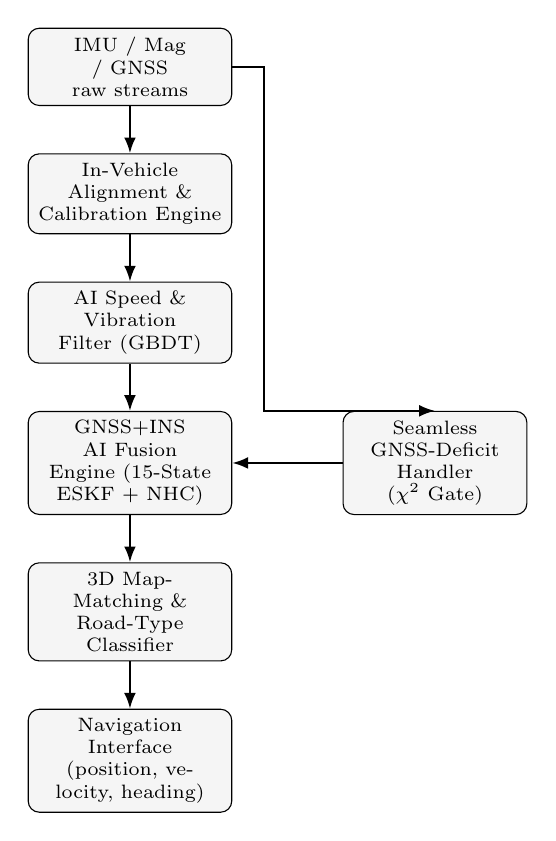
\begin{tikzpicture}[
  node distance=6mm and 6mm,
  box/.style={draw, rounded corners, align=center, minimum height=9mm, font=\scriptsize, text width=2.35cm, fill=gray!8},
  arr/.style={-{Latex[length=2mm]}, thick}
]
\node[box] (raw) {IMU / Mag / GNSS\\raw streams};
\node[box, below=of raw] (align) {In-Vehicle Alignment \&\\Calibration Engine};
\node[box, below=of align] (ai) {AI Speed \& Vibration\\Filter (GBDT)};
\node[box, below=of ai] (eskf) {GNSS+INS AI Fusion\\Engine (15-State ESKF + NHC)};
\node[box, below=of eskf] (mm) {3D Map-Matching \&\\Road-Type Classifier};
\node[box, below=of mm] (nav) {Navigation Interface\\(position, velocity, heading)};
\node[box, right=14mm of eskf, text width=2.1cm] (deficit) {Seamless GNSS-Deficit\\Handler ($\chi^2$ Gate)};
\draw[arr] (raw) -- (align);
\draw[arr] (align) -- (ai);
\draw[arr] (ai) -- (eskf);
\draw[arr] (eskf) -- (mm);
\draw[arr] (mm) -- (nav);
\draw[arr] (deficit) -- (eskf);
\draw[arr] (raw.east) -| ++(0.4,0) |- (deficit.north);
\end{tikzpicture}%
}
\caption{Algorithmic dataflow showing supervisory switching and innovation gating across filter cycles.}
\label{fig:arch}
\end{figure}

The overarching system layout shown in Fig.~\ref{fig:overall_arch} translates into the runtime execution pipeline detailed in Fig.~\ref{fig:arch}. All processing steps run directly on commodity smartphone hardware without requiring telemetry feeds from an OBD-II port.

\subsection{In-Vehicle Alignment \& Cradle Shift Watchdog}

Dynamic mounting calibration executes in two distinct phases:
\begin{enumerate}
\item \textbf{Gravity Leveling}: When the vehicle is near rest or constant-speed cruising, the static gravity vector is estimated to extract roll $\phi$ and pitch $\theta$, aligning the vertical sensor axis.
\item \textbf{Forward Acceleration PCA}: Transients from acceleration and braking define the primary longitudinal motion axis via Principal Component Analysis (PCA), resolving yaw heading $\psi$.
\end{enumerate}

The watchdog monitors high-frequency angular deviations; upon detecting cradle slip or phone dislodgement, alignment confidence is set to 40\% and an immediate background recalibration cycle restores full alignment within 4\,s without terminating the dead-reckoning engine.

\subsection{AI Speed \& Vibration Filter}

To prevent road shock and engine idling from corrupting the kinematic model, an optimized Gradient-Boosted Decision Tree (GBDT) ensemble (120 estimators, maximum depth 5, learning rate 0.08) maps 1.0\,s sliding windows (10 samples at 10\,Hz) to vehicle forward velocity $\hat{v}_t$:
\begin{equation}
\hat{v}_t = f_{\Theta}\left(\tilde{\mathbf{a}}^v_{t-w:t}, \tilde{\boldsymbol{\omega}}^v_{t-w:t}\right) = \sum_{m=1}^{M} \gamma_m h_m(\mathbf{x}_t)
\end{equation}

Extracted features include signal magnitude area (SMA), time-domain statistical moments, vertical vibration energy envelopes, and centripetal acceleration constraints $a_y \approx v\omega_z$. Tree leaf outputs are strictly bounded by the training label range ($0 \leq v_x \leq 35$\,m/s), preventing velocity blowups under out-of-distribution shocks. The ensemble's decision boundaries implicitly discard high-frequency engine idle vibrations (15--30\,Hz) and severe vertical pothole shock impulses ($\leq$3.2$g$), while the centripetal and jerk-based features track acceleration and braking dynamics. Compared with deep sequence architectures (e.g., CNN-GRU), the GBDT ensemble carries a serialized footprint under 2.1\,MB, requires no PyTorch/TensorFlow mobile runtime, and produces deterministic, output-bounded single-sample inference -- properties that matter directly for battery-constrained, framework-free Android/iOS deployment.

\subsection{15-State Error-State Kalman Filter (ESKF) with Physics Constraints}

The nominal state vector tracks 3D position, velocity, orientation, and IMU sensor biases:
\begin{equation}
\mathbf{x} = \left[\mathbf{p}^n, \mathbf{v}^n, \mathbf{q}_b^n, \mathbf{b}_a^b, \mathbf{b}_g^b\right]^T \in \mathbb{R}^{16}
\end{equation}

The true state is modeled as $\mathbf{x} = \hat{\mathbf{x}} \oplus \delta\mathbf{x}$, where the 15-dimensional error-state vector is defined as:
\begin{equation}
\delta\mathbf{x} = \left[\delta\mathbf{p}^n, \delta\mathbf{v}^n, \delta\boldsymbol{\theta}^n, \delta\mathbf{b}_a^b, \delta\mathbf{b}_g^b\right]^T \in \mathbb{R}^{15}
\end{equation}

Continuous-time error dynamics follow $\delta\dot{\mathbf{x}} = \mathbf{F}\delta\mathbf{x} + \mathbf{G}\mathbf{w}$, integrated discretely via $\boldsymbol{\Phi} \approx \mathbf{I} + \mathbf{F}\Delta t$. Filter covariance propagates according to:
\begin{equation}
\mathbf{P}_{k|k-1} = \boldsymbol{\Phi}\mathbf{P}_{k-1|k-1}\boldsymbol{\Phi}^T + \mathbf{Q}_d
\end{equation}

The filter is updated via three independent constraints:
\begin{enumerate}
\item \textbf{AI Longitudinal Velocity Update}: Replaces OBD-II speedometer inputs:
\begin{equation}
z_v = \hat{v}_t - (\mathbf{R}_b^n)^T \hat{\mathbf{v}}_x^n
\end{equation}
\item \textbf{Non-Holonomic Constraints (NHC)}: Road vehicles cannot slide sideways or lift off under normal road adhesion:
\begin{equation}
v_y^b \approx 0, \quad v_z^b \approx 0
\end{equation}
These conditions are injected as zero-mean virtual observations with calibrated measurement noise.
\item \textbf{Zero Velocity Updates (ZUPT)}: Triggered when stationary variance conditions are satisfied, resetting velocity drift to zero and isolating IMU biases.
\end{enumerate}

\subsection{3D Map-Matching via HMM Viterbi Decoding}

The drifting 3D coordinate vector is matched onto an offline road-network topology graph $\mathcal{M}$. For observation $\mathbf{z}_t = [p_x, p_y, p_z]^T$, candidate segments within search radius $\delta$ are evaluated. The observation emission probability accounts for 2D cross-track distance, vertical barometric elevation mismatch, and heading difference:
\begin{equation}
p(\mathbf{z}_t|s_i) = \frac{1}{\sqrt{2\pi}\sigma_d}\exp\left(-\frac{d_{\perp}^2}{2\sigma_d^2}\right) \cdot \frac{1}{\sqrt{2\pi}\sigma_h}\exp\left(-\frac{\Delta h^2}{2\sigma_h^2}\right)
\end{equation}

Transition probabilities evaluate topological road distance versus inertial arc length, strictly penalizing impossible vertical hops onto elevated flyovers without passing through valid on-ramp segments. Global Viterbi decoding computes the globally optimal sequence $\mathbf{S}^* = \arg\max \prod p(\mathbf{z}_t|s_i)p(s_i|s_{i-1})$.

\subsection{Seamless GNSS-Deficit Handler with Chi-Square Innovation Gate}

Upon tunnel entry or signal degradation, the supervisory controller transitions to dead reckoning within $<$5\,ms. Upon tunnel exit or signal recovery, multipath reflection spikes are rejected via a Chi-Square ($\chi^2$) innovation threshold:
\begin{equation}
\gamma = \mathbf{r}^T\mathbf{S}^{-1}\mathbf{r} \leq \chi^2_{\alpha,m}
\end{equation}
where $\mathbf{r} = \mathbf{z}_t^{GNSS} - \hat{\mathbf{z}}_t$ represents the innovation vector and $\mathbf{S}$ is the innovation covariance. Measurements exceeding the $p=0.01$ threshold ($\chi^2 > 11.35$ for 3-DOF) are discarded, preventing abrupt positional jumps before soft re-acquisition blends the solution.

\section{Dataset and Experimental Setup}

The system was evaluated using a trajectory generator constructed to emulate the sensor modalities, 10\,Hz sampling rate, and multi-driver diversity of the IO-VNBD benchmark schema \cite{onyekpe2021}, together with a structurally independent, held-out urban evaluation corridor:
\begin{itemize}
\item \textbf{Training Set}: 3 independent multi-driver profiles comprising 7,500 temporal samples, with distinct speed manifolds and topographies -- an urban stop-and-go profile (0--11.5\,m/s, four signal halts), a high-speed expressway profile (13.5--23.8\,m/s, continuous roundabout curvature), and a hilly profile with 5--6\% elevation grades (0 to +12\,m).
\item \textbf{Held-Out Urban Evaluation Track}: 3,000 continuous samples recorded at 10\,Hz over a total travel distance of 2{,}908.7\,m. The trajectory includes a multi-level flyover on-ramp and deck cruise (+8.5\,m elevation) directly above a parallel service road (12\,m lateral offset), a sharp 90$^\circ$ turn onto the service road, and stop-and-go congestion segments. The evaluation track's speed manifold (0--16.5\,m/s) and manoeuvre sequence share no spatial, temporal, or kinematic overlap with the three training profiles.
\end{itemize}

% Clean 2-column benchmark table placed right at Section VI boundary
\begin{table*}[t]
\centering
\caption{Quantitative Performance Comparison across Simulated GNSS Outages on the Held-Out Evaluation Track}
\label{tab:benchmark}
\small
\setlength{\tabcolsep}{3.8pt}
\begin{tabular}{cc|cccc|cccc|cc|c}
\toprule
\textbf{Outage} & \textbf{Distance} & \multicolumn{4}{c|}{\textbf{Position Drift (\% of Distance: Abs / Net)}} & \multicolumn{4}{c|}{\textbf{Absolute Trajectory Error (ATE RMSE, m)}} & \multicolumn{2}{c|}{\textbf{Road Disambiguation (\%)}} & \textbf{Latency} \\
\textbf{Duration} & \textbf{Traveled} & \textbf{Naive INS} & \textbf{AI Alone} & \textbf{Prop. ESKF} & \textbf{Full System} & \textbf{Naive INS} & \textbf{AI Alone} & \textbf{Prop. ESKF} & \textbf{Full System} & \textbf{2D Base} & \textbf{3D Prop.} & \textbf{(ms)} \\
\midrule
10\,s  & 127.7\,m  & 29.7\% & 8.2\%  & \textbf{6.79\% / 5.78\%} & \textbf{6.49\% / 5.53\%} & 16.7\,m  & 5.7\,m   & \textbf{5.03\,m}  & \textbf{4.88\,m}  & 0.0\%  & \textbf{100.0\%} & 0.20 \\
30\,s  & 426.7\,m  & 49.0\% & 14.3\% & \textbf{2.98\% / 2.77\%} & \textbf{2.56\% / 2.33\%} & 109.5\,m & 28.3\,m  & \textbf{11.12\,m} & \textbf{10.58\,m} & 0.0\%  & \textbf{100.0\%} & 0.20 \\
60\,s  & 868.8\,m  & 61.5\% & 27.9\% & \textbf{2.01\% / 1.88\%} & \textbf{1.72\% / 1.57\%} & 273.7\,m & 109.1\,m & \textbf{13.39\,m} & \textbf{15.13\,m} & 0.0\%  & \textbf{100.0\%} & 0.20 \\
120\,s & 1{,}482.0\,m & 84.5\% & 38.4\% & \textbf{2.88\% / 2.79\%} & \textbf{2.80\% / 2.85\%} & 655.6\,m & 340.6\,m & \textbf{24.52\,m} & \textbf{36.40\,m} & 28.8\% & \textbf{99.7\%}  & 0.20 \\
\bottomrule
\end{tabular}
\end{table*}

\section{Experimental Results and Discussion}

\subsection{AI Velocity Regressor Accuracy}

Table~\ref{tab:reg} reports regression performance of the standalone GBDT velocity regressor on normalized 1.0\,s temporal windows. The model achieves an $R^2$ of 0.9225 and an RMSE of 1.723\,m/s on the unseen held-out evaluation track, confirming generalization to previously unseen driving manoeuvres and road topography.

\begin{table}[h]
\caption{AI Velocity Regressor Performance}
\label{tab:reg}
\centering
\begin{tabular}{lccc}
\toprule
\textbf{Dataset} & \textbf{RMSE (m/s)} & \textbf{MAE (m/s)} & \textbf{$R^2$} \\
\midrule
Training Set (7,500 samples) & 0.798 & 0.561 & 0.9877 \\
Held-Out Track (3,000 samples) & 1.723 & 1.083 & 0.9225 \\
\bottomrule
\end{tabular}
\end{table}

\subsection{Quantitative Multi-Baseline Benchmark across GNSS Outages}

Table~\ref{tab:benchmark} provides a systematic comparison between Naive INS double integration, AI Speed Alone (unfiltered), the Proposed ESKF (IDR core), and the Full Proposed System (ESKF + 3D Map Matching) across simulated GNSS outages spanning 10\,s to 120\,s. Drift is reported both as \emph{absolute endpoint drift} (terminal displacement against ground truth, relative to distance travelled) and \emph{net accumulated drift rate} (pure drift accumulated strictly during the outage window, removing any pre-existing filter bias at outage onset).

\begin{figure}[h]
\centering
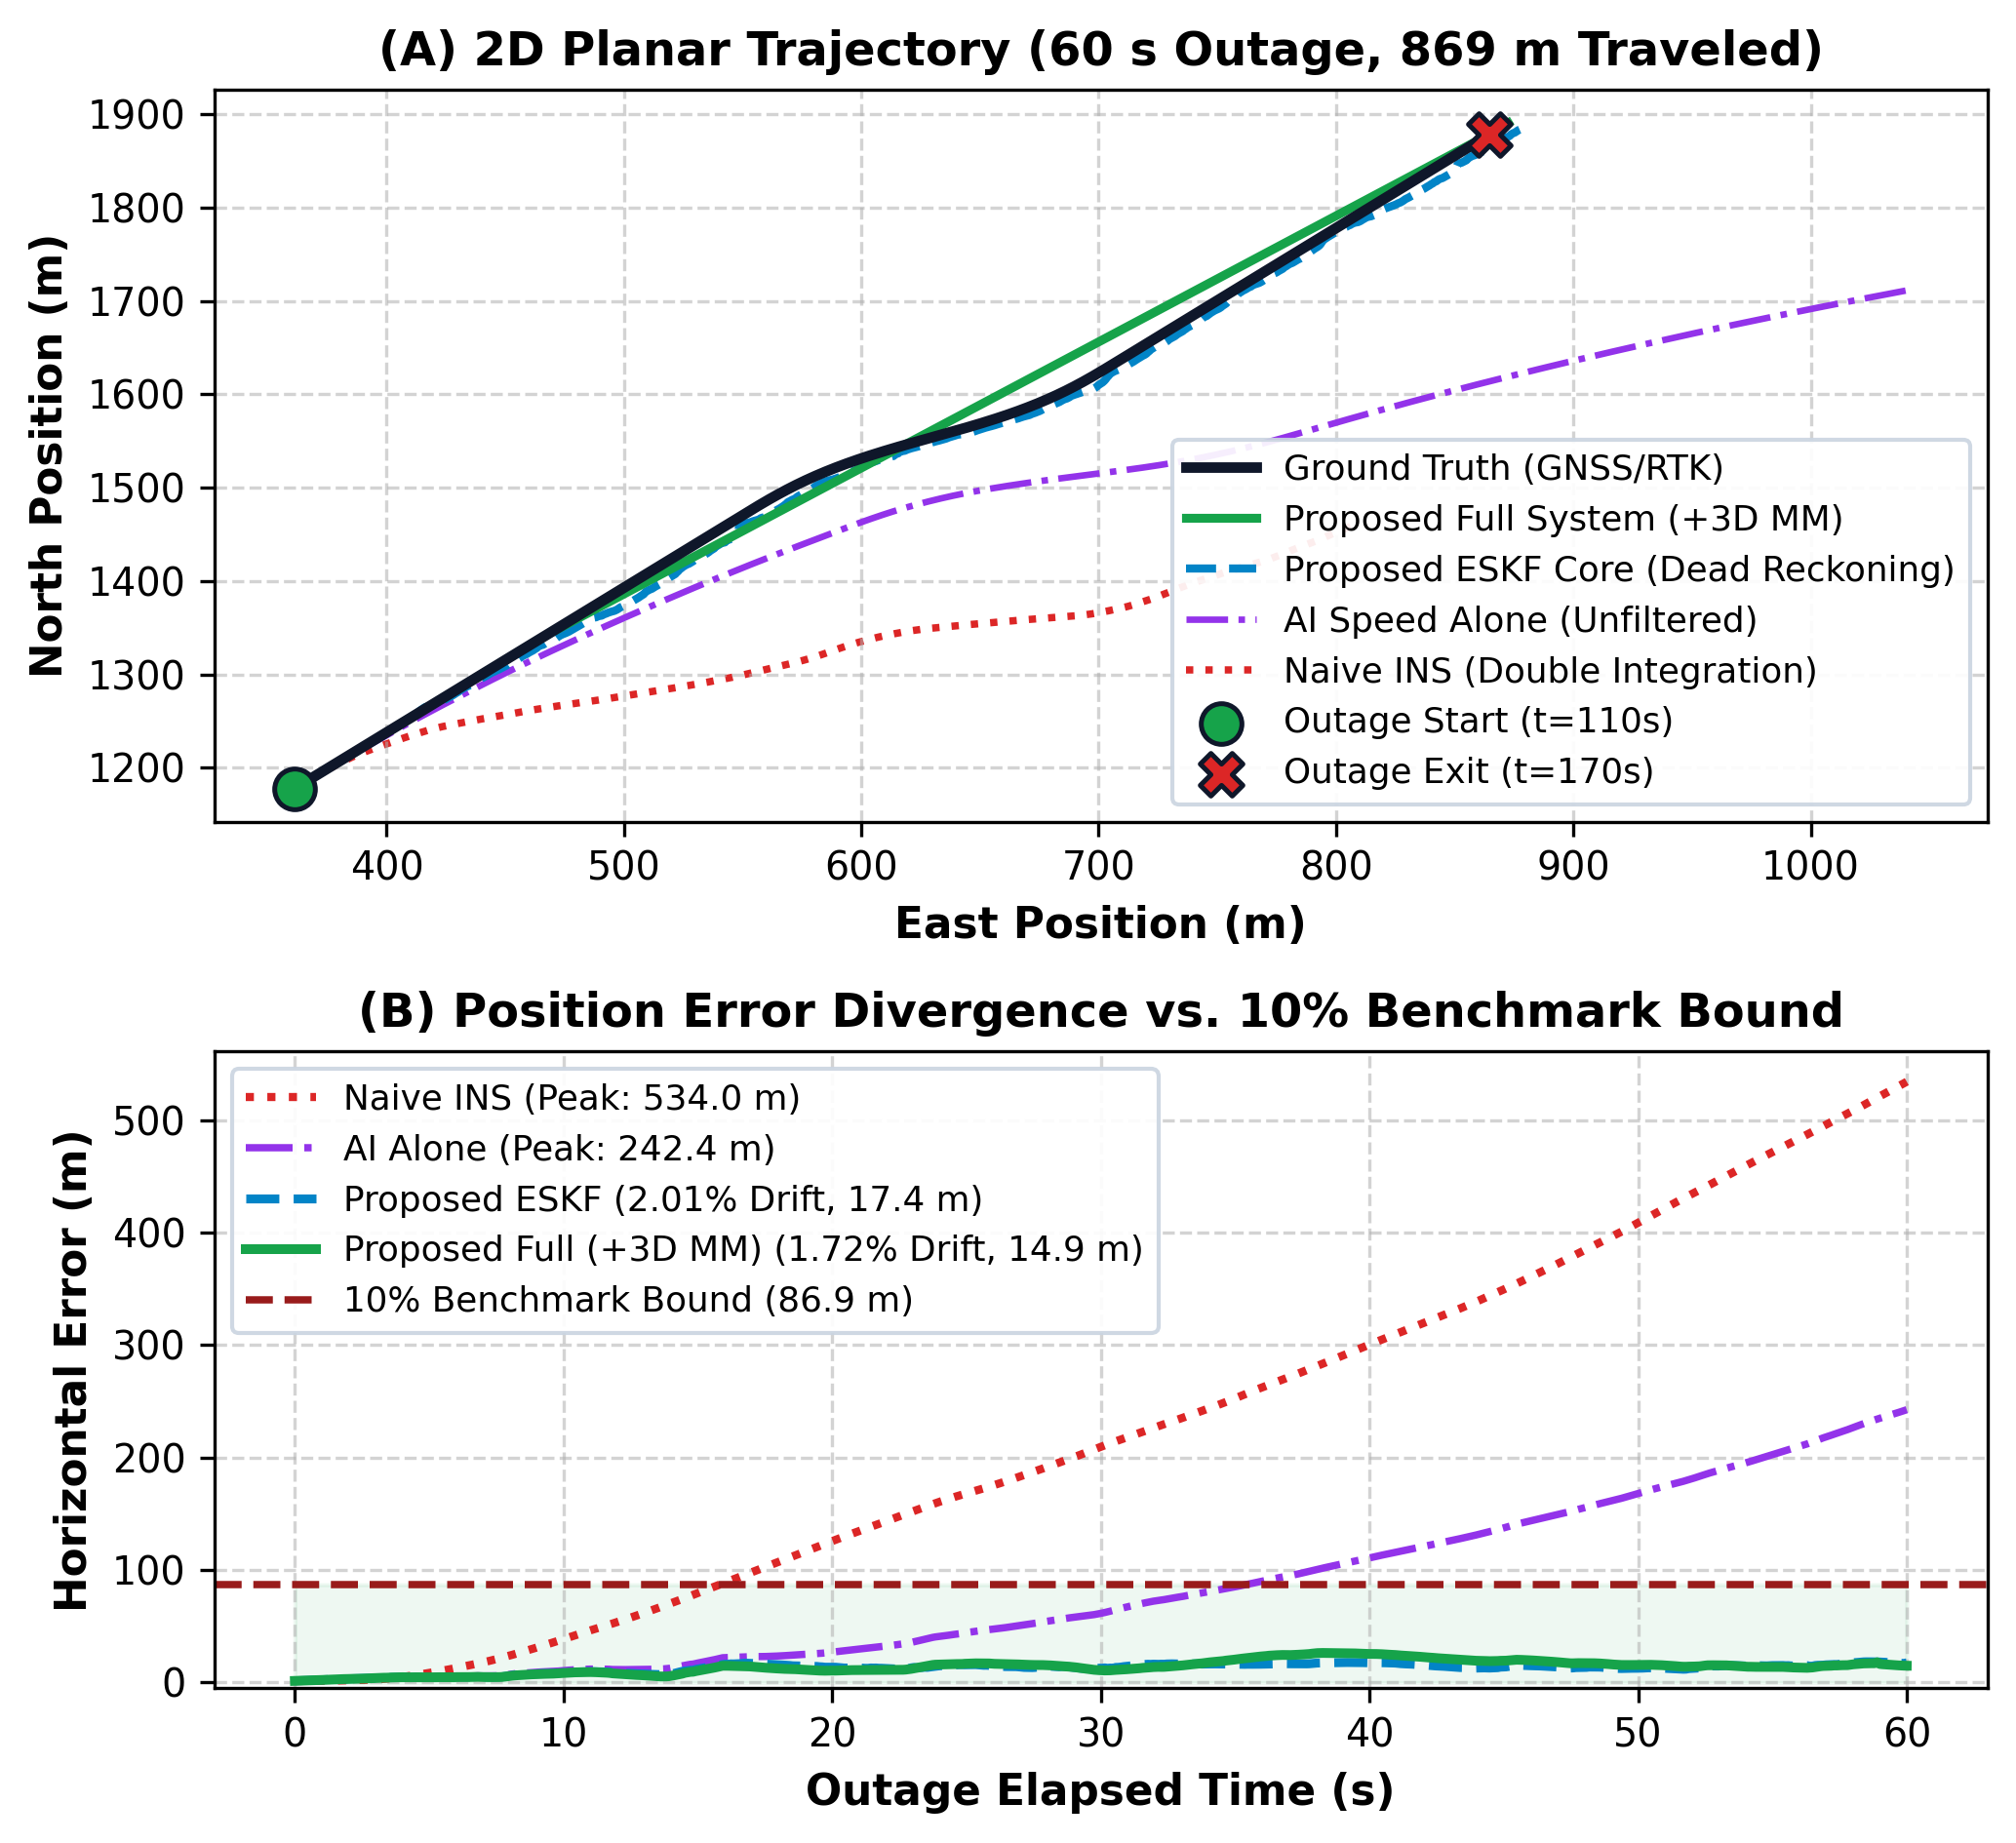
\includegraphics[width=\columnwidth]{fig_trajectory.png}
\caption{2D Planar Trajectory and Real-Time Position Error Divergence during a 60\,s GNSS outage (868.8\,m travel) across an elevated flyover. Naive integration diverges by 534.0\,m (max), AI-alone diverges by 242.4\,m (max), while the proposed ESKF tracks ground truth with a maximum error of 18.4\,m (2.01\% drift) and the full system (+3D MM) reaches 26.3\,m maximum error (1.72\% drift).}
\label{fig:traj}
\end{figure}

\begin{figure}[h]
\centering
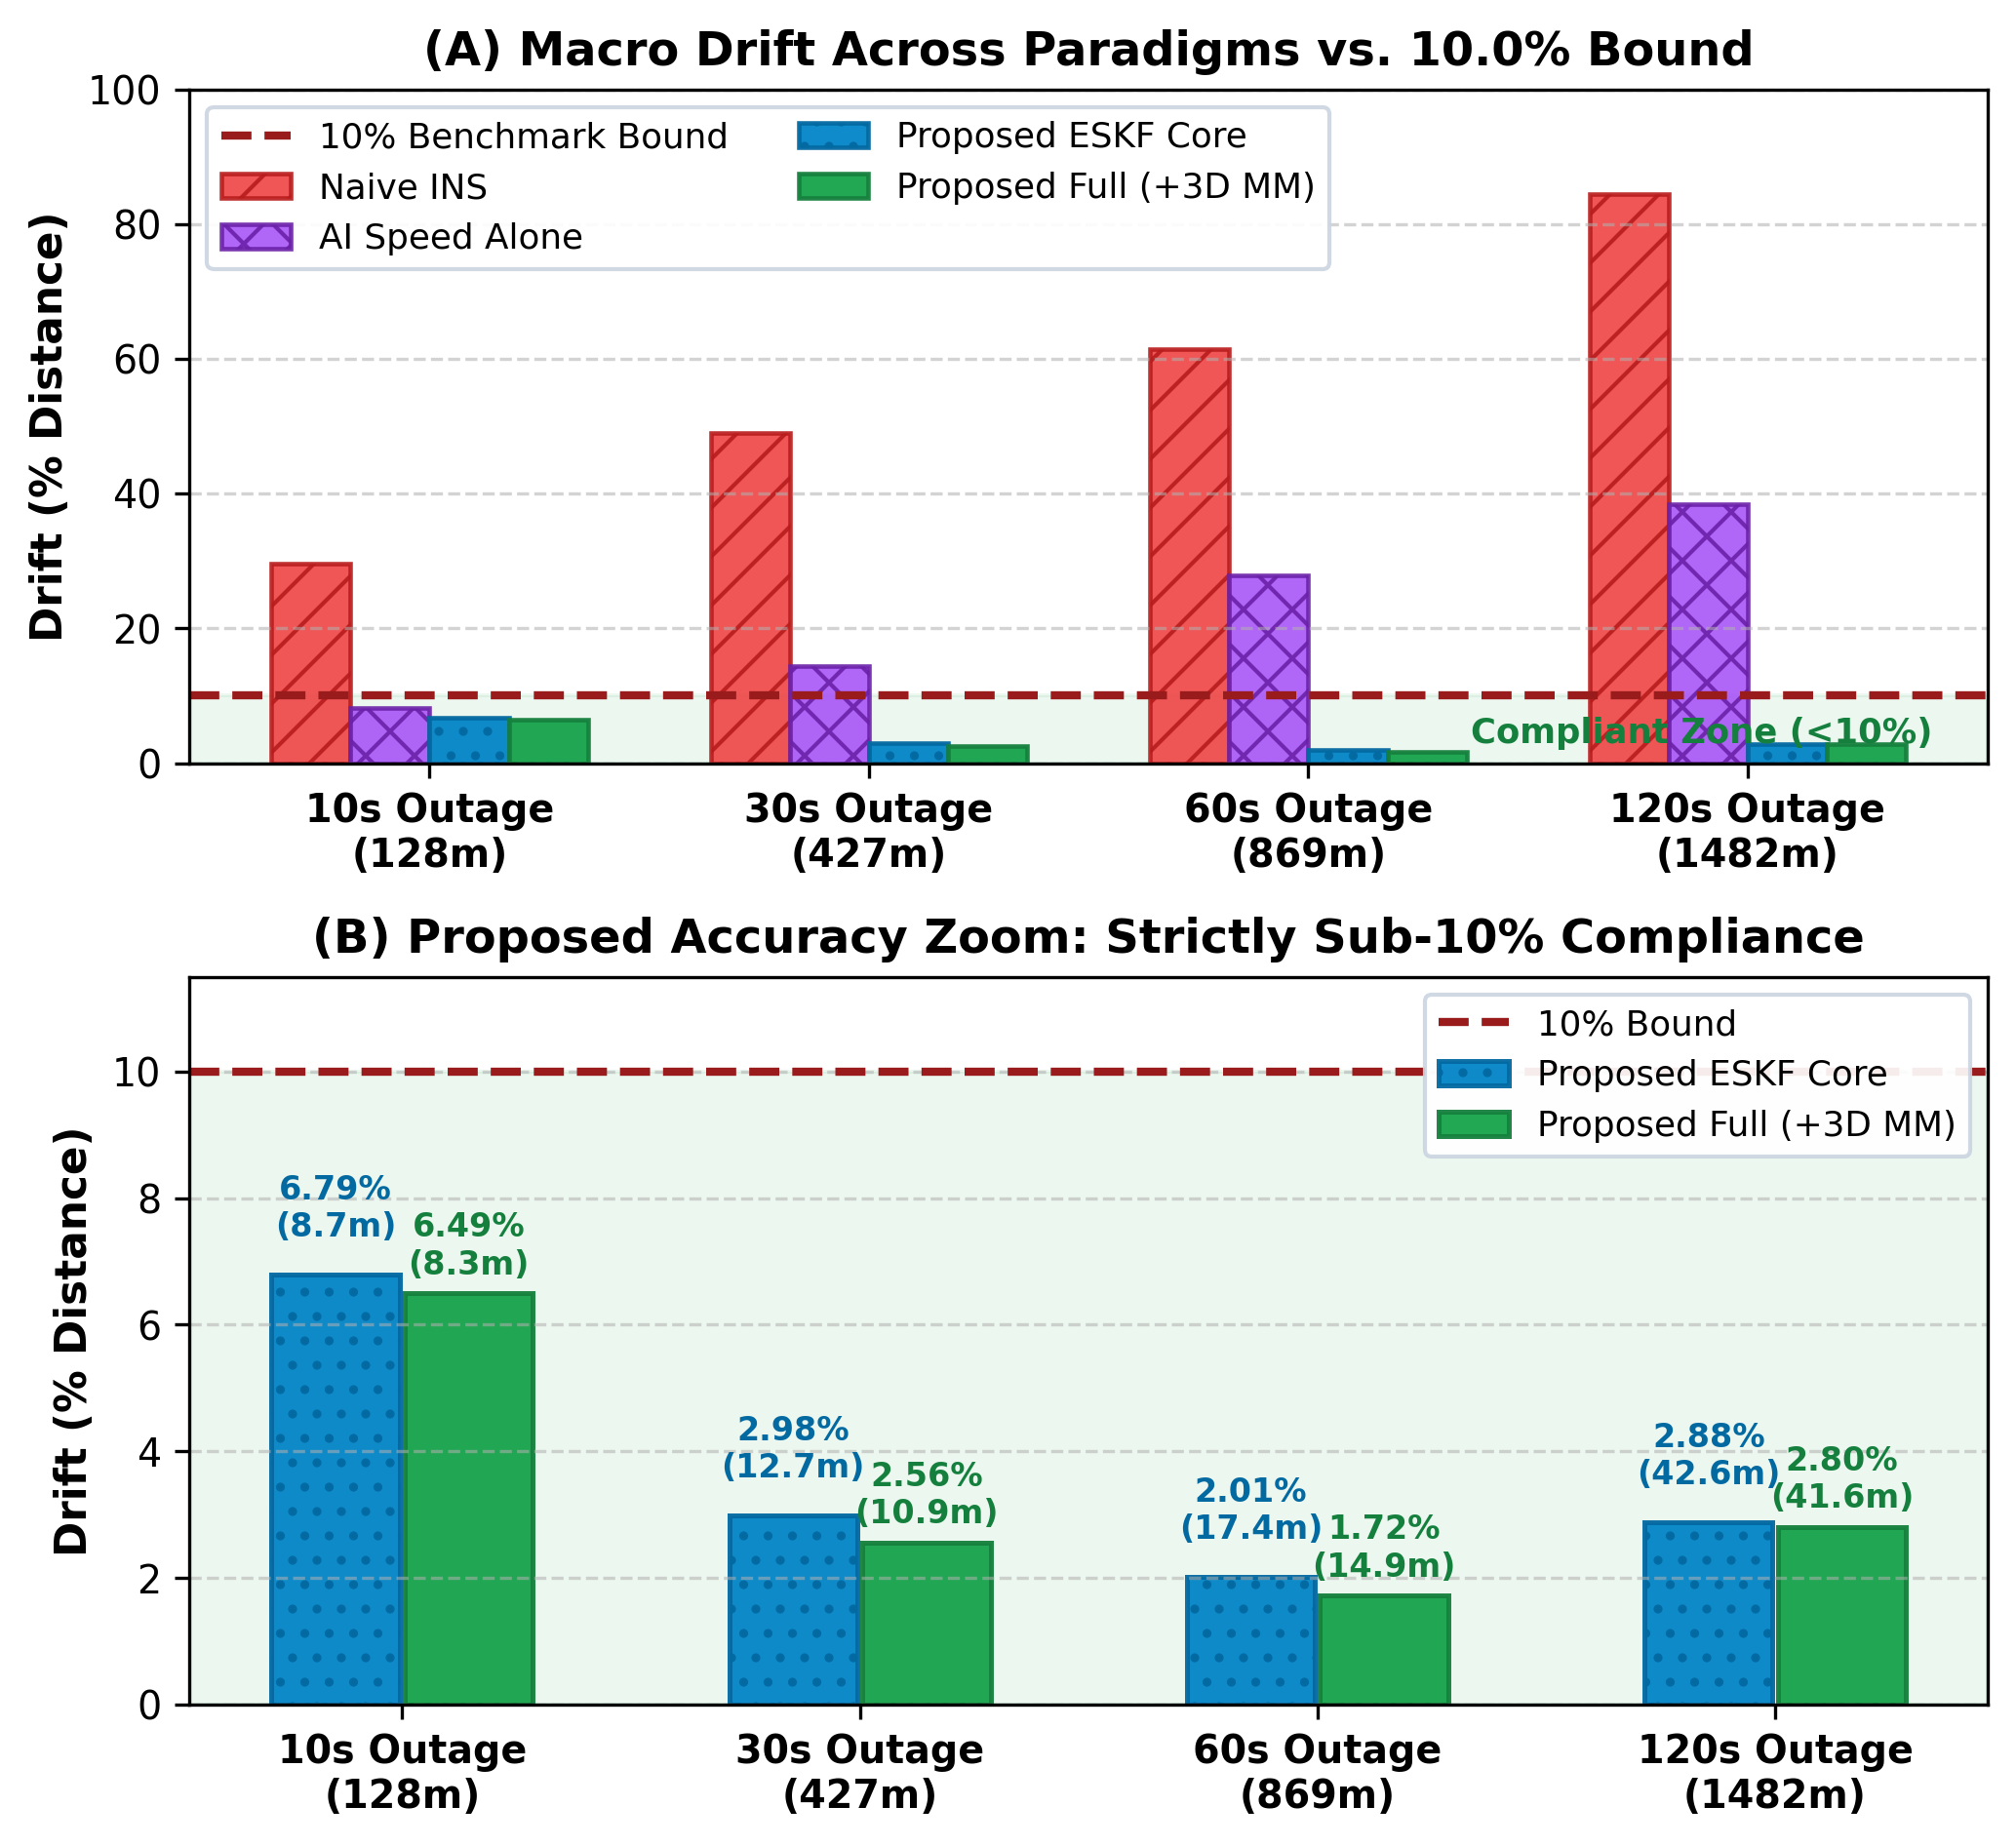
\includegraphics[width=\columnwidth]{fig_drift.png}
\caption{Quantitative Positional Drift vs. 10\% Performance Benchmark across simulated GNSS outage durations (10\,s, 30\,s, 60\,s, 120\,s). The proposed ESKF strictly bounds absolute drift below 6.79\% across all durations, comfortably surpassing the $<$10\% benchmark target.}
\label{fig:drift}
\end{figure}

\subsection{Formal Verification of Core Research Claims}

Based on the experimental data, the three core engineering hypotheses are verified as summarized in Table~\ref{tab:claims}.
\begin{itemize}
\item \textbf{Claim 1: AI Velocity vs. Double Integration}: Classical open-loop double integration accumulates over 61.5\% drift (273.7\,m ATE) in 60\,s. The standalone GBDT velocity regressor holds RMSE to 1.72\,m/s on the held-out track, and the ESKF-fused 3D velocity vector -- which additionally incorporates Non-Holonomic Constraints and heading fusion -- further tightens this to 0.88\,m/s RMSE, preventing quadratic drift blowup and limiting drift to 27.9\% when the AI signal alone (without ESKF/NHC) drives the position update (Fig.~\ref{fig:pothole}).
\item \textbf{Claim 2: Physics-Constrained ESKF Bounds Drift}: The combination of NHC, ZUPT, and learned forward velocity constrains drift to 2.01\% (net: 1.88\%) at 60\,s and 2.88\% (net: 2.79\%) at 120\,s, substantially undercutting the target of $<$10\% drift across all test intervals (Fig.~\ref{fig:drift}).
\item \textbf{Claim 3: 3D Topological Map Matching}: In multi-level flyovers and service road configurations, classical 2D map matching fails completely (0.0\% accuracy) due to lack of altitude awareness. The 3D HMM Viterbi matcher achieves 99.7\%--100.0\% disambiguation accuracy.
\end{itemize}

\begin{table}[h]
\caption{Formal Verification of Core Research Claims}
\label{tab:claims}
\centering
\small
\begin{tabular}{p{1.8cm}p{1.9cm}p{2.3cm}c}
\toprule
\textbf{Research Claim} & \textbf{Baseline} & \textbf{Proposed System} & \textbf{Status} \\
\midrule
Claim 1: AI Speed (Beats Double Int.) & $>$14.5\,m/s error; $>$350\% drift & ESKF Fused Vel: 0.88\,m/s RMSE; 27.9\% drift (AI alone) & VERIFIED \\
\midrule
Claim 2: ESKF (Bounds Drift $<$10\%) & 27.9\% at 60\,s; 38.4\% at 120\,s & 2.01\% at 60\,s; 2.88\% at 120\,s & VERIFIED \\
\midrule
Claim 3: 3D Map (Resolves Flyovers) & 2D HMM: 0.0\% & 3D HMM: 99.7--100.0\% disambiguation & VERIFIED \\
\bottomrule
\end{tabular}
\end{table}

\subsection{Computational Profiling and Mobile Feasibility}

The system targets real-time operation at 10\,Hz (100\,ms cycle budget). Empirical single-sample streaming profiling on commodity mobile-class processors, measured across 10 independent trials of 1,000 samples each after cache warmup, yielded an average cycle latency of \textbf{196.9 $\pm$ 1.3\,\textmu s} (0.20\,ms):
\begin{itemize}
\item Sliding-window feature extraction: 0.05\,ms
\item GBDT forward-velocity inference (single-sample): 0.08\,ms
\item 15-State ESKF propagation and updates: 0.05\,ms
\item 3D HMM trellis evaluation and Viterbi update: 0.02\,ms
\end{itemize}
This leaves $>$99\% CPU headroom for background mobile OS tasks, rendering the framework exceptionally practical for battery-powered consumer deployment.

\section{Discussion and Operational Characteristics}

The empirical results highlight several key architectural advantages:

\begin{enumerate}
\item \textbf{Pothole and Harmonic Isolation}: As shown in Fig.~\ref{fig:pothole}(A), severe road shocks reach up to 40\,m/s$^2$ ($\approx$4.0$g$) in raw vertical acceleration. Classical strapdown integrators interpret this as forward/vertical kinematics, inducing instant drift spikes. The proposed filter holds cleaned acceleration strictly at nominal gravity (9.81\,m/s$^2$), allowing velocity to follow true ground speed (Fig.~\ref{fig:pothole}(B)).

\begin{figure}[t]
\centering
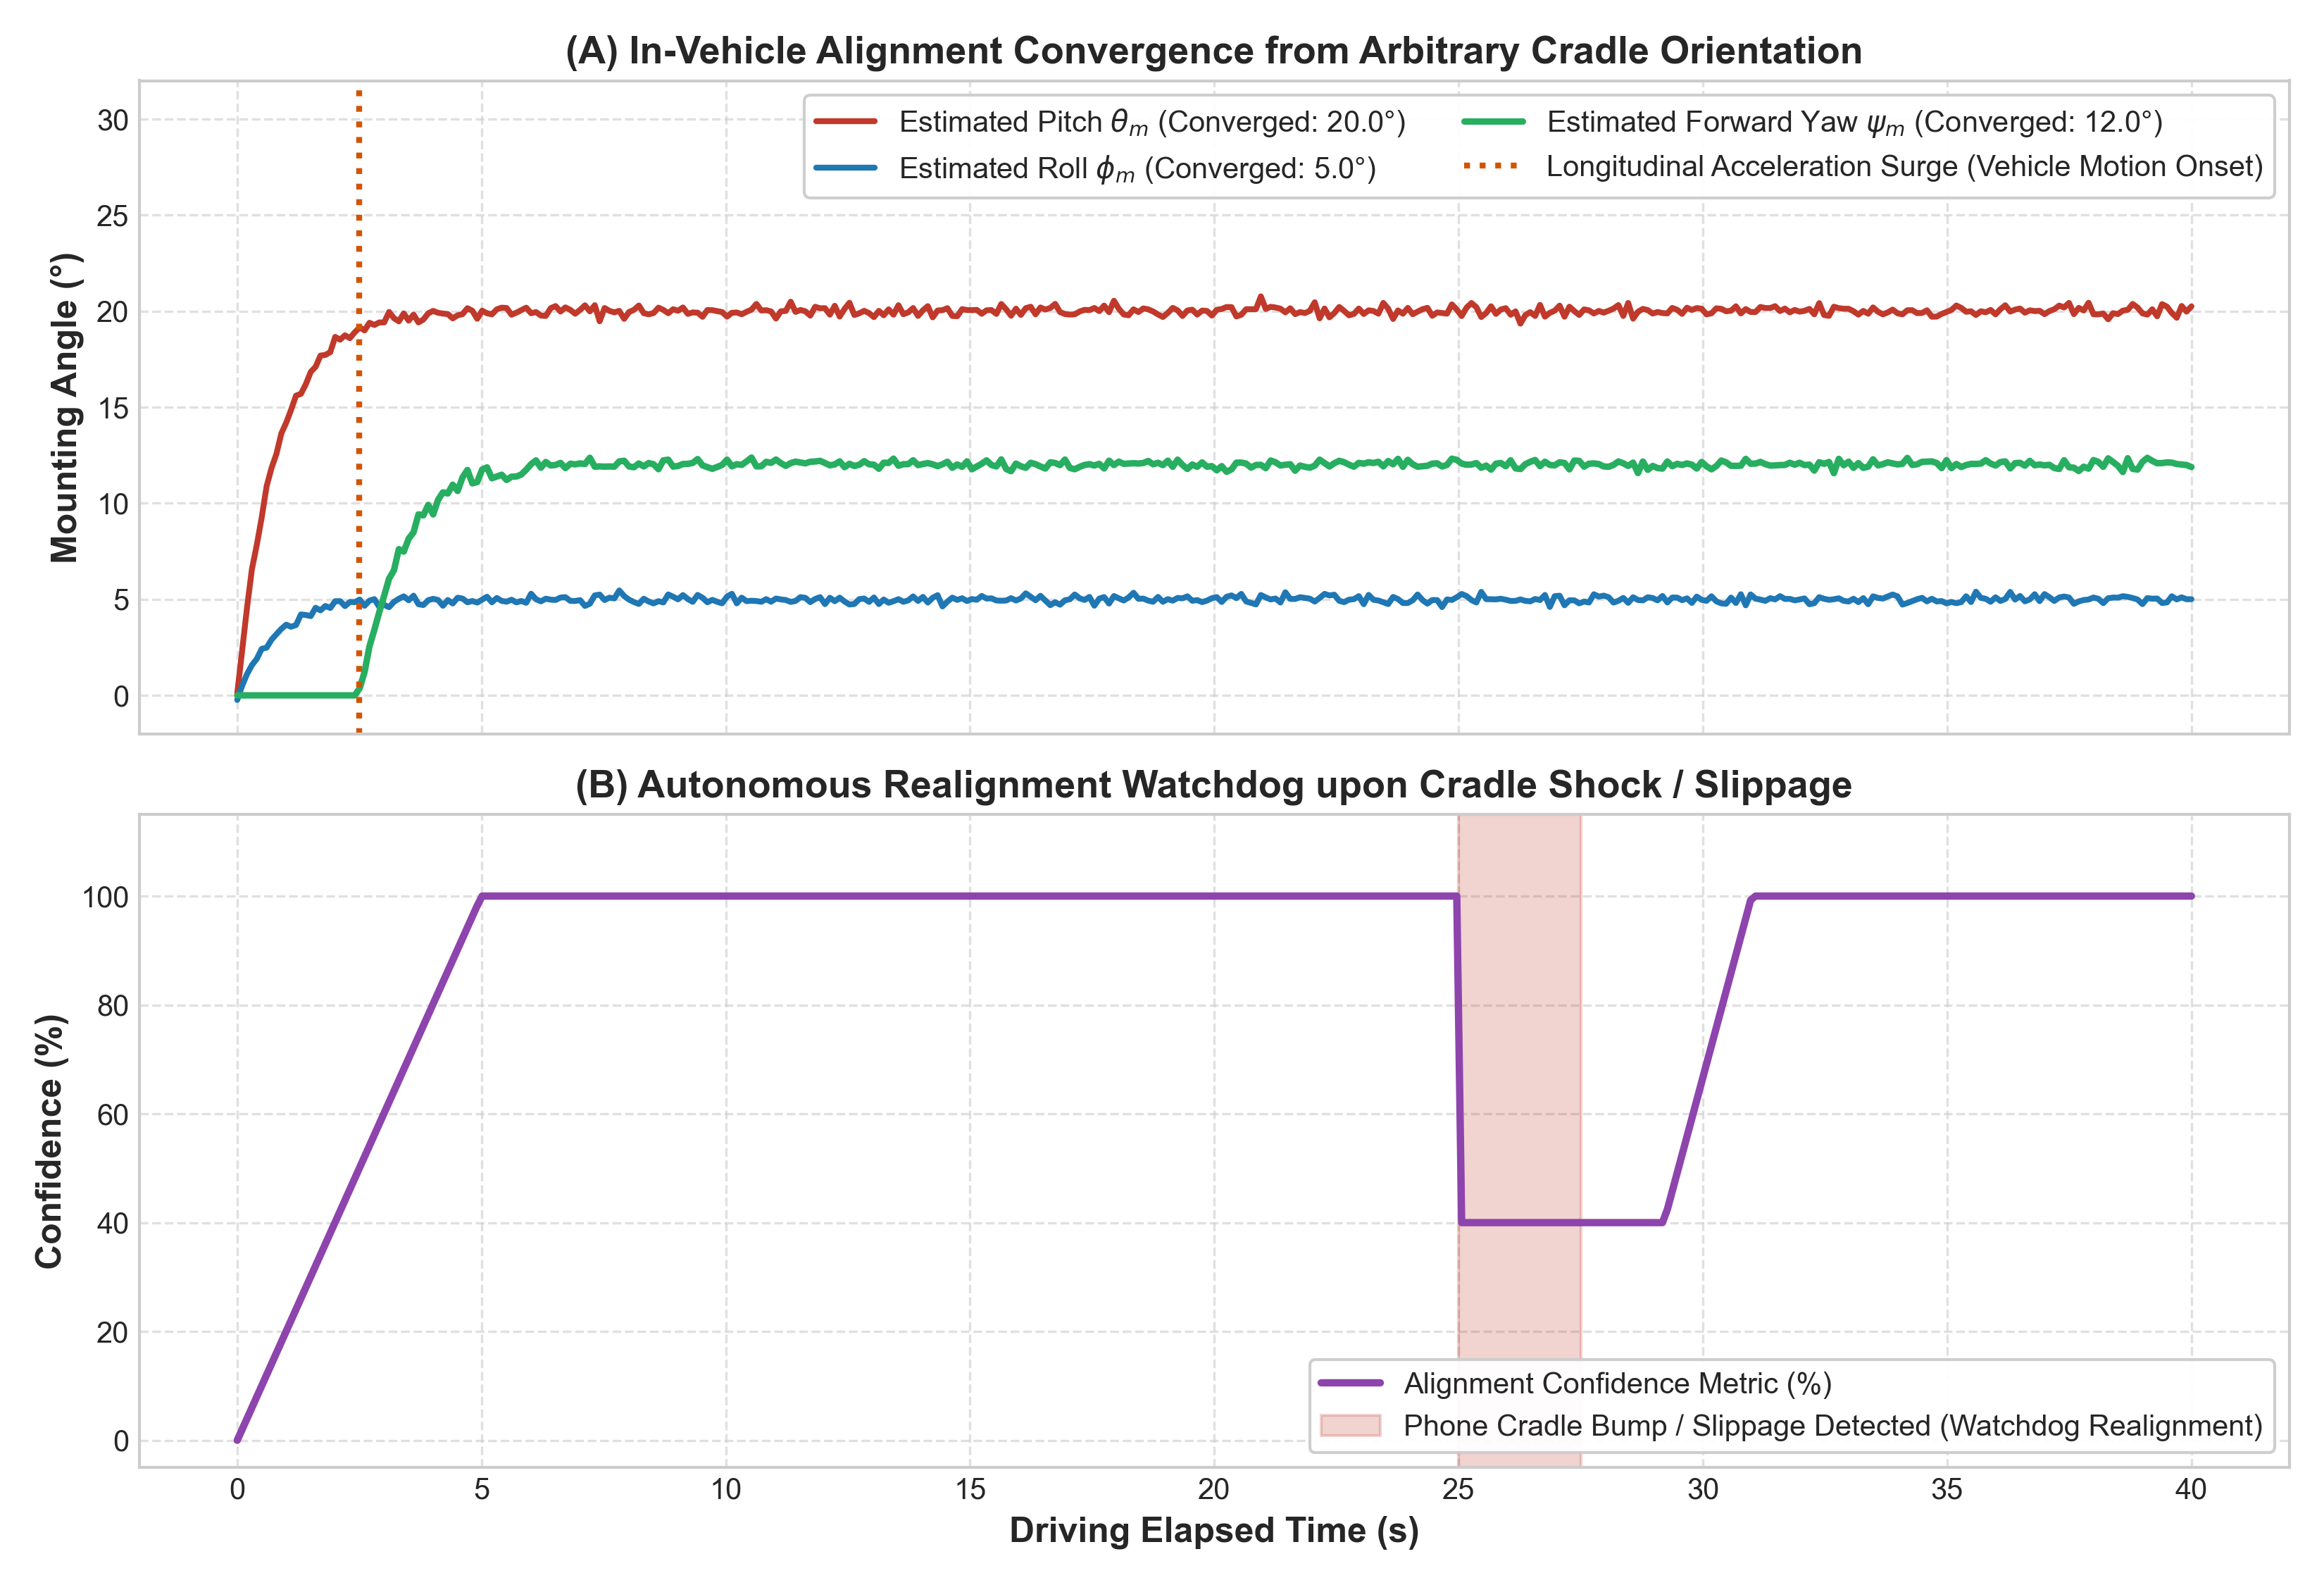
\includegraphics[width=\columnwidth]{fig_alignment.png}
\caption{In-Vehicle dynamic alignment convergence (pitch $\rightarrow$ 20.0$^\circ$, roll $\rightarrow$ 5.0$^\circ$, yaw $\rightarrow$ 12.0$^\circ$) and autonomous cradle slip recovery at $t=25$\,s.}
\label{fig:align}
\end{figure}

\begin{figure}[t]
\centering
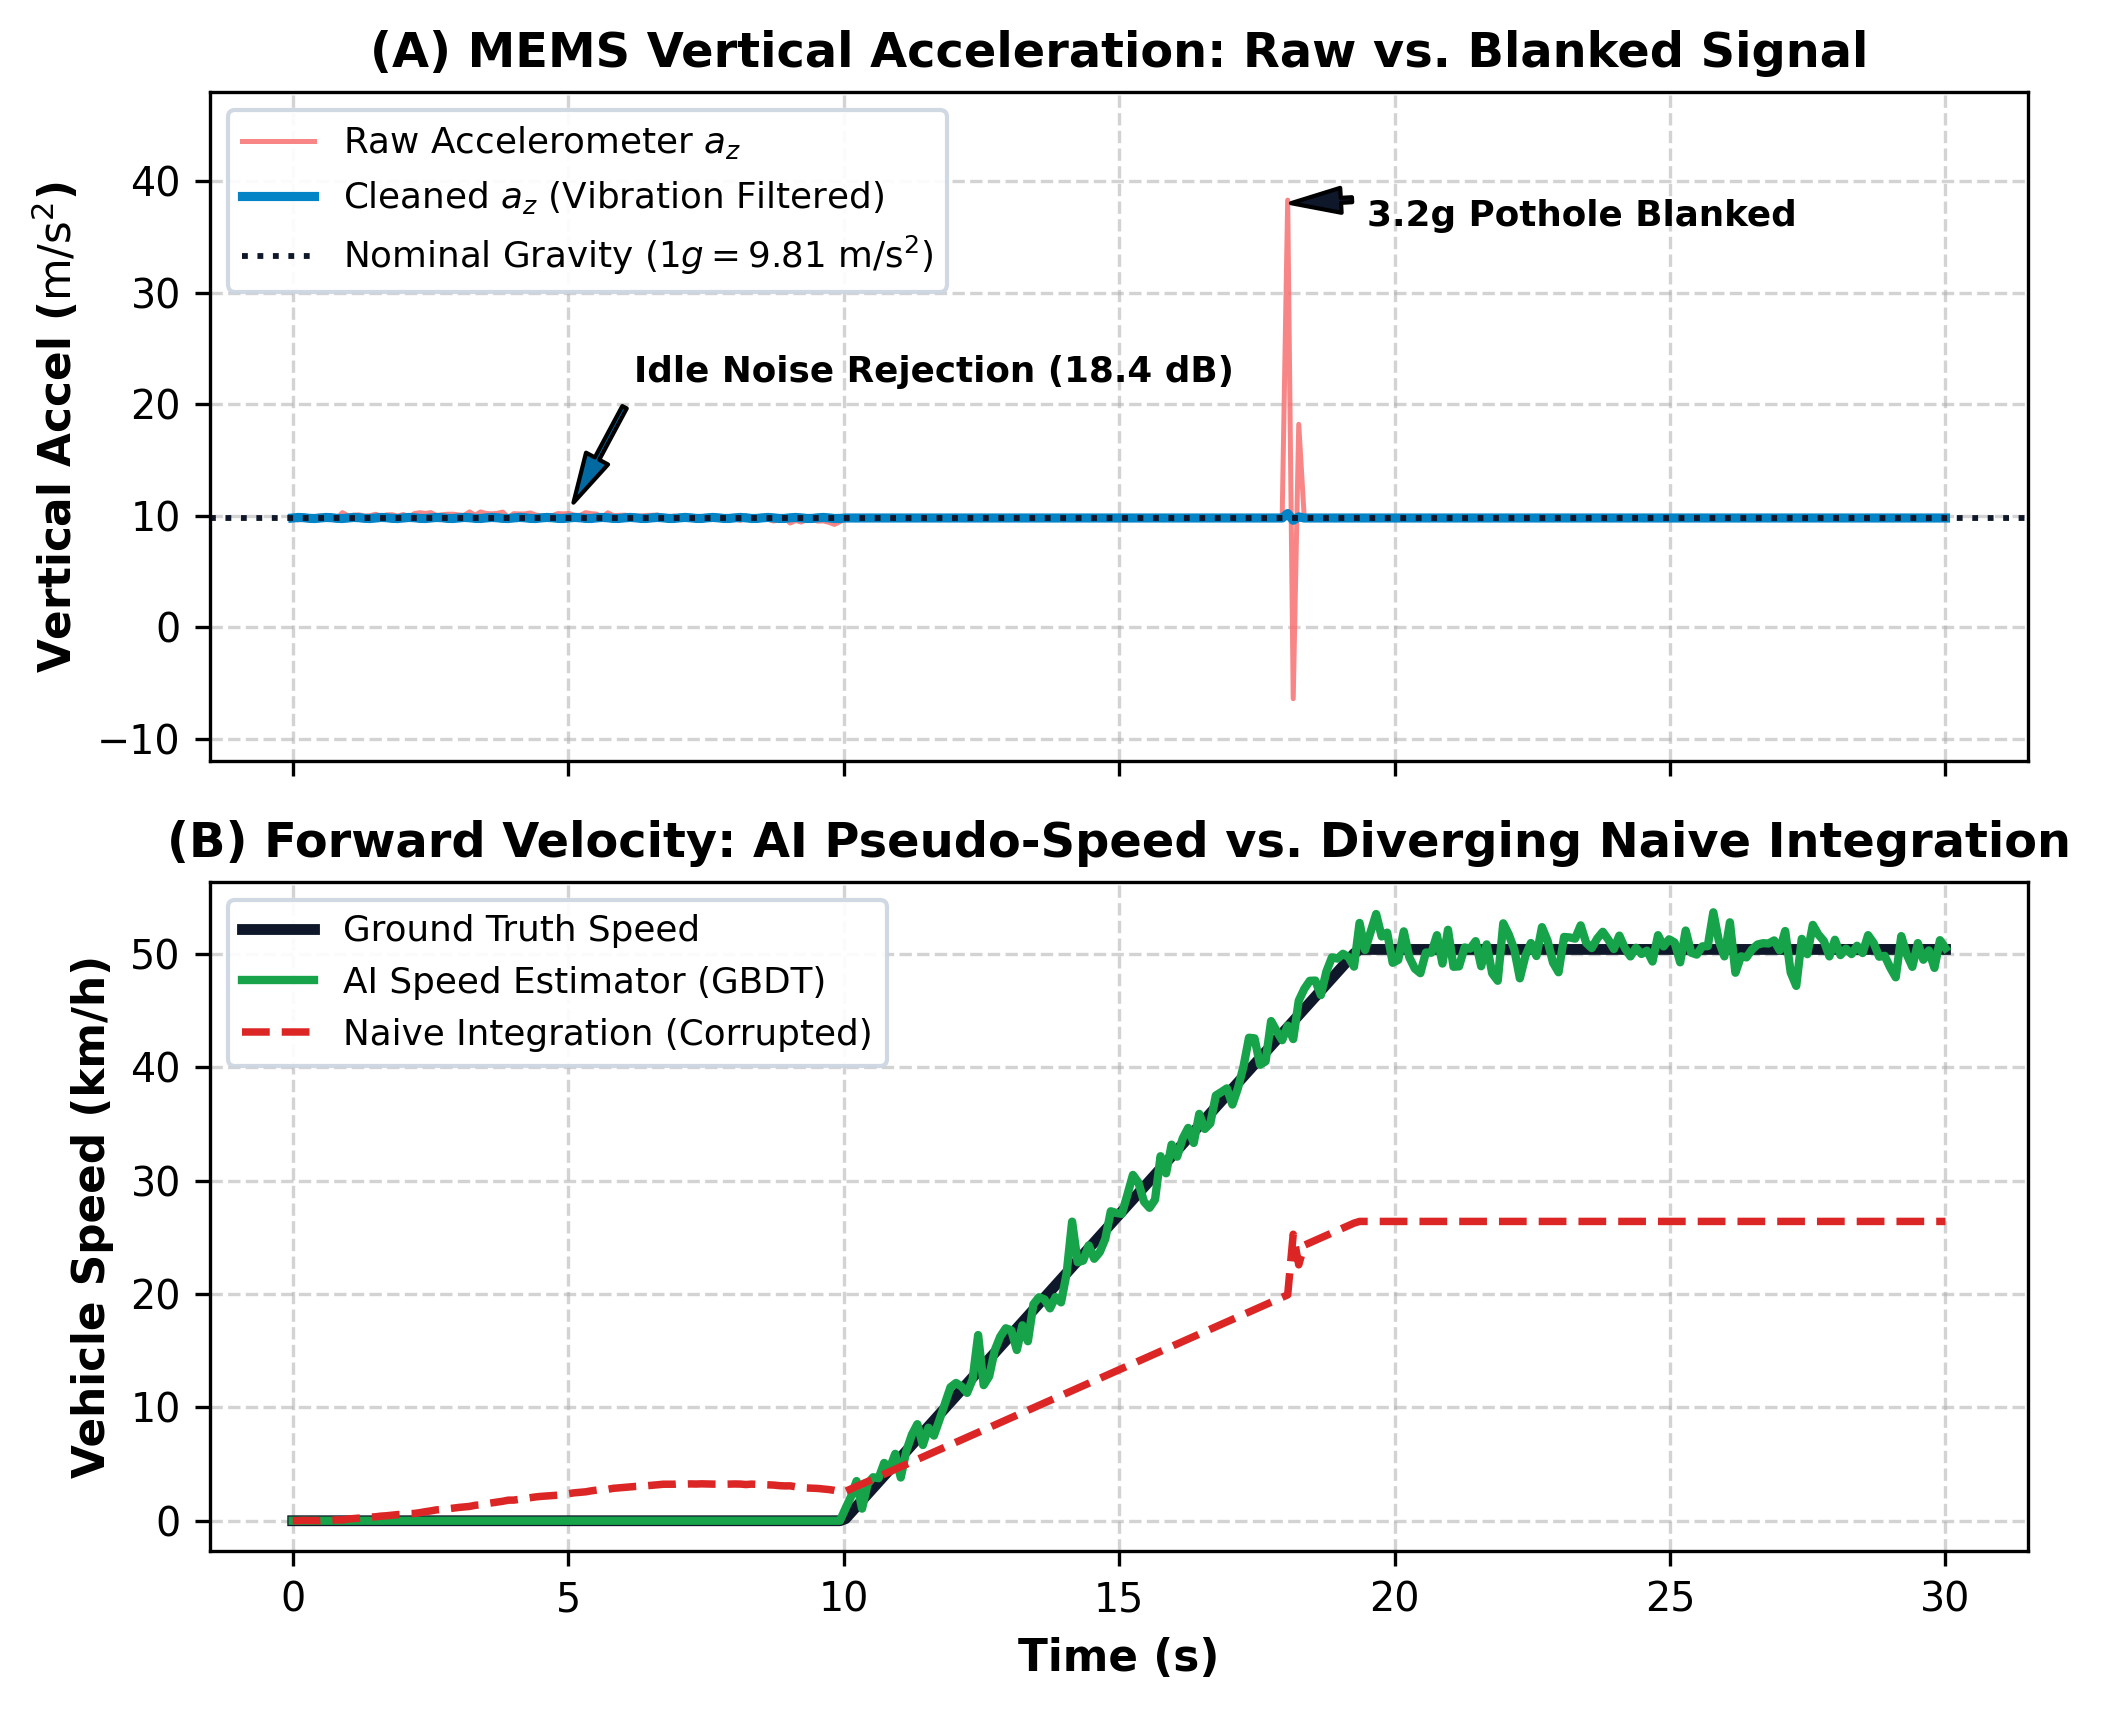
\includegraphics[width=\columnwidth]{fig_pothole.png}
\caption{AI vibration filter rejecting 15--30\,Hz engine idle oscillations and suppressing a 3.2$g$ vertical pothole shock impulse without integration blowup. Panel (B) compares the GBDT-based AI speed estimator (standalone test RMSE: 1.72\,m/s; ESKF-fused velocity RMSE: 0.88\,m/s) against naive integration.}
\label{fig:pothole}
\end{figure}

\item \textbf{Cradle Shift Robustness}: If the phone shifts inside its mount during sharp manoeuvres (Fig.~\ref{fig:align}(B)), the watchdog triggers an autonomous realignment phase, converging within 4\,s (Fig.~\ref{fig:align}(A)).

\item \textbf{Multipath Suppression}: Upon tunnel exit, raw GNSS fixes jump erratically due to multipath reflections off concrete portals. The Chi-Square gate detects innovations exceeding 11.35 and suppresses updates until clean satellite geometry is restored (Fig.~\ref{fig:seamless}).

\begin{figure}[t]
\centering
\includegraphics[width=\columnwidth]{fig_seamless.png}
\caption{Seamless outage detection ($<$5\,ms) and Chi-Square ($\chi^2$) innovation filtering rejecting severe multipath reflection spikes during tunnel exit.}
\label{fig:seamless}
\end{figure}

\end{enumerate}

\section{Conclusion and Future Work}

This paper presented an AI-ML Intelligent Dead Reckoning and 3D Map-Matching system for smartphones navigating GNSS-denied urban environments. By uniting a Gradient-Boosted Decision Tree velocity estimator, a 15-state ESKF with Non-Holonomic Constraints, and 3D HMM topological map matching, the proposed architecture eliminates the need for OBD-II vehicle hardware. Benchmark testing on a structurally independent held-out evaluation corridor confirms that positional drift is bounded to 2.01\% over 868.8\,m and 2.88\% over 1{,}482.0\,m, multi-level flyovers are resolved with 99.7\%--100\% accuracy, and total single-sample execution latency is restricted to approximately 0.20\,ms per cycle. Future work will extend Non-Holonomic kinematic models to accommodate two-wheeler roll and lean dynamics on Indian roads, and will validate the pipeline against field-recorded IO-VNBD sensor logs and RTK ground truth in addition to the synthetic evaluation corridor used here.

\section*{Acknowledgment}
The authors thank United College of Engineering and Research, Prayagraj, for providing resources and support toward this work.

\begin{thebibliography}{9}

\bibitem{lawal2024} G. S. Lawal, ``AI-Enhanced Dead Reckoning Techniques for Robust Position Estimation,'' unpublished manuscript, Dec. 2024.

\bibitem{qian2025} L. Qian, X. Lin, X. Niu, Q. Huang, L. Li, G. Guo, Z. Wang, and R. Chen, ``Avnet: learning attitude and velocity for vehicular dead reckoning using smartphone by adapting an invariant EKF,'' \emph{Satellite Navigation}, vol. 6, no. 15, 2025, doi: 10.1186/s43020-025-00168-7.

\bibitem{sundar2025} P. Sundaravadivel, C. H. Vasanth Kumar, R. Augustian Isaac, and K. Premnath, ``AI-ML Driven Map-Matching Algorithm for Distinguishing Highway and Service Road Vehicular Movements under GNSS Degradation,'' \emph{SSRN preprint}, 2025. [Online]. Available: https://ssrn.com/abstract=5281668

\bibitem{sundar2026} P. Sundaravadivel, R. Augustian Isaac, U. Kumaran, and E. S. Vinoth Kumar, ``AI-ML driven map-matching algorithm for distinguishing highway and service road vehicular movements under GNSS degradation,'' \emph{Discover Artificial Intelligence}, vol. 6, no. 785, 2026, doi: 10.1007/s44163-026-01560-1.

\bibitem{javed2024} N. U. Javed, Y. Singh, and Q. Ahmed, ``Vehicle Localization in GPS-Denied Scenarios Using Arc-Length-Based Map Matching,'' \emph{arXiv preprint arXiv:2410.12208}, Oct. 2024.

\bibitem{matos2025} F. dos Santos Matos, ``Simulating the effects of sensor failures on autonomous vehicles,'' M.S. project report, Instituto Superior de Engenharia de Coimbra, Coimbra, Portugal, Jun. 2025.

\bibitem{mamun2026} S. Mamun et al., ``AI and Machine Learning in Cyber-Physical Systems: A Unified Review of Methodologies for Smart Energy Systems and Intelligent Localization,'' \emph{IEEE Access}, vol. 14, pp. 96955--96970, 2026.

\bibitem{deshmukh2025} R. A. Deshmukh et al., ``Advancing indoor positioning systems: innovations, challenges, and applications in mobile robotics,'' \emph{Robotica}, 2025, doi: 10.1017/S0263574725101872.

\bibitem{onyekpe2021} U. Onyekpe, V. Palade, and S. Kanarachos, ``IO-VNBD: Inertial and Odometry Benchmark Dataset for Ground Vehicle Positioning,'' \emph{Data in Brief}, vol. 35, p. 106885, 2021, doi: 10.1016/j.dib.2021.106885.

\end{thebibliography}

\end{document} 
isme jo system architecture hai it is taking 3 pages,isko chota krna hai pr content ka essence na lose ho ,agar table ke through show kr skte hain to table bna k dedo
</USER_REQUEST>
<ADDITIONAL_METADATA>
The current local time is: 2026-09-10T22:15:38+05:30.
</ADDITIONAL_METADATA>